\subsection{Flight Plan II - Fixed Waypoints}
%\textcolor{red}{Peng's flight plan}


\subsubsection{Motivation}
%In some applications, the \ac{UAV} is required to achieve some pre-defined locations. During the flight to the locations, the \ac{UAV} is supposed to avoid obstacles. Under this circumstance, a flight plan with fixed way points is required.
The two main objective or performance indexes are as follows:
\begin{enumerate}
\item Distance.
\item Fewer number of collisions.
\end{enumerate}

We believe that if there exists a logic where the \ac{UAV} can follow the fixed way points while avoiding the obstacles, then we have a larger possibility to achieve a longer distance. 

Additionally, in practice, the \ac{UAV} is usually supposed to fly to different locations other than moving randomly. Due to these reasons, we offer another flight plan which is the fixed flight plan.


\subsubsection{Strategy}
Actually, there can be many strategies which may achieve the above-mentioned flight plan. One of the strategies is denoted in Fig.~\ref{f:fp}.

\begin{figure}
\centering
\psfrag{p0} 		[][]  {$p_0$}
\psfrag{p1} 		[][]  {$p_1$}
\psfrag{p2} 		[][]  {$p_2$}
\psfrag{p3} 		[][]  {$p_3$}
\psfrag{p4} 		[][]  {$p_4$}

%\includegraphics[scale=0.6]{DIA/MM.eps}
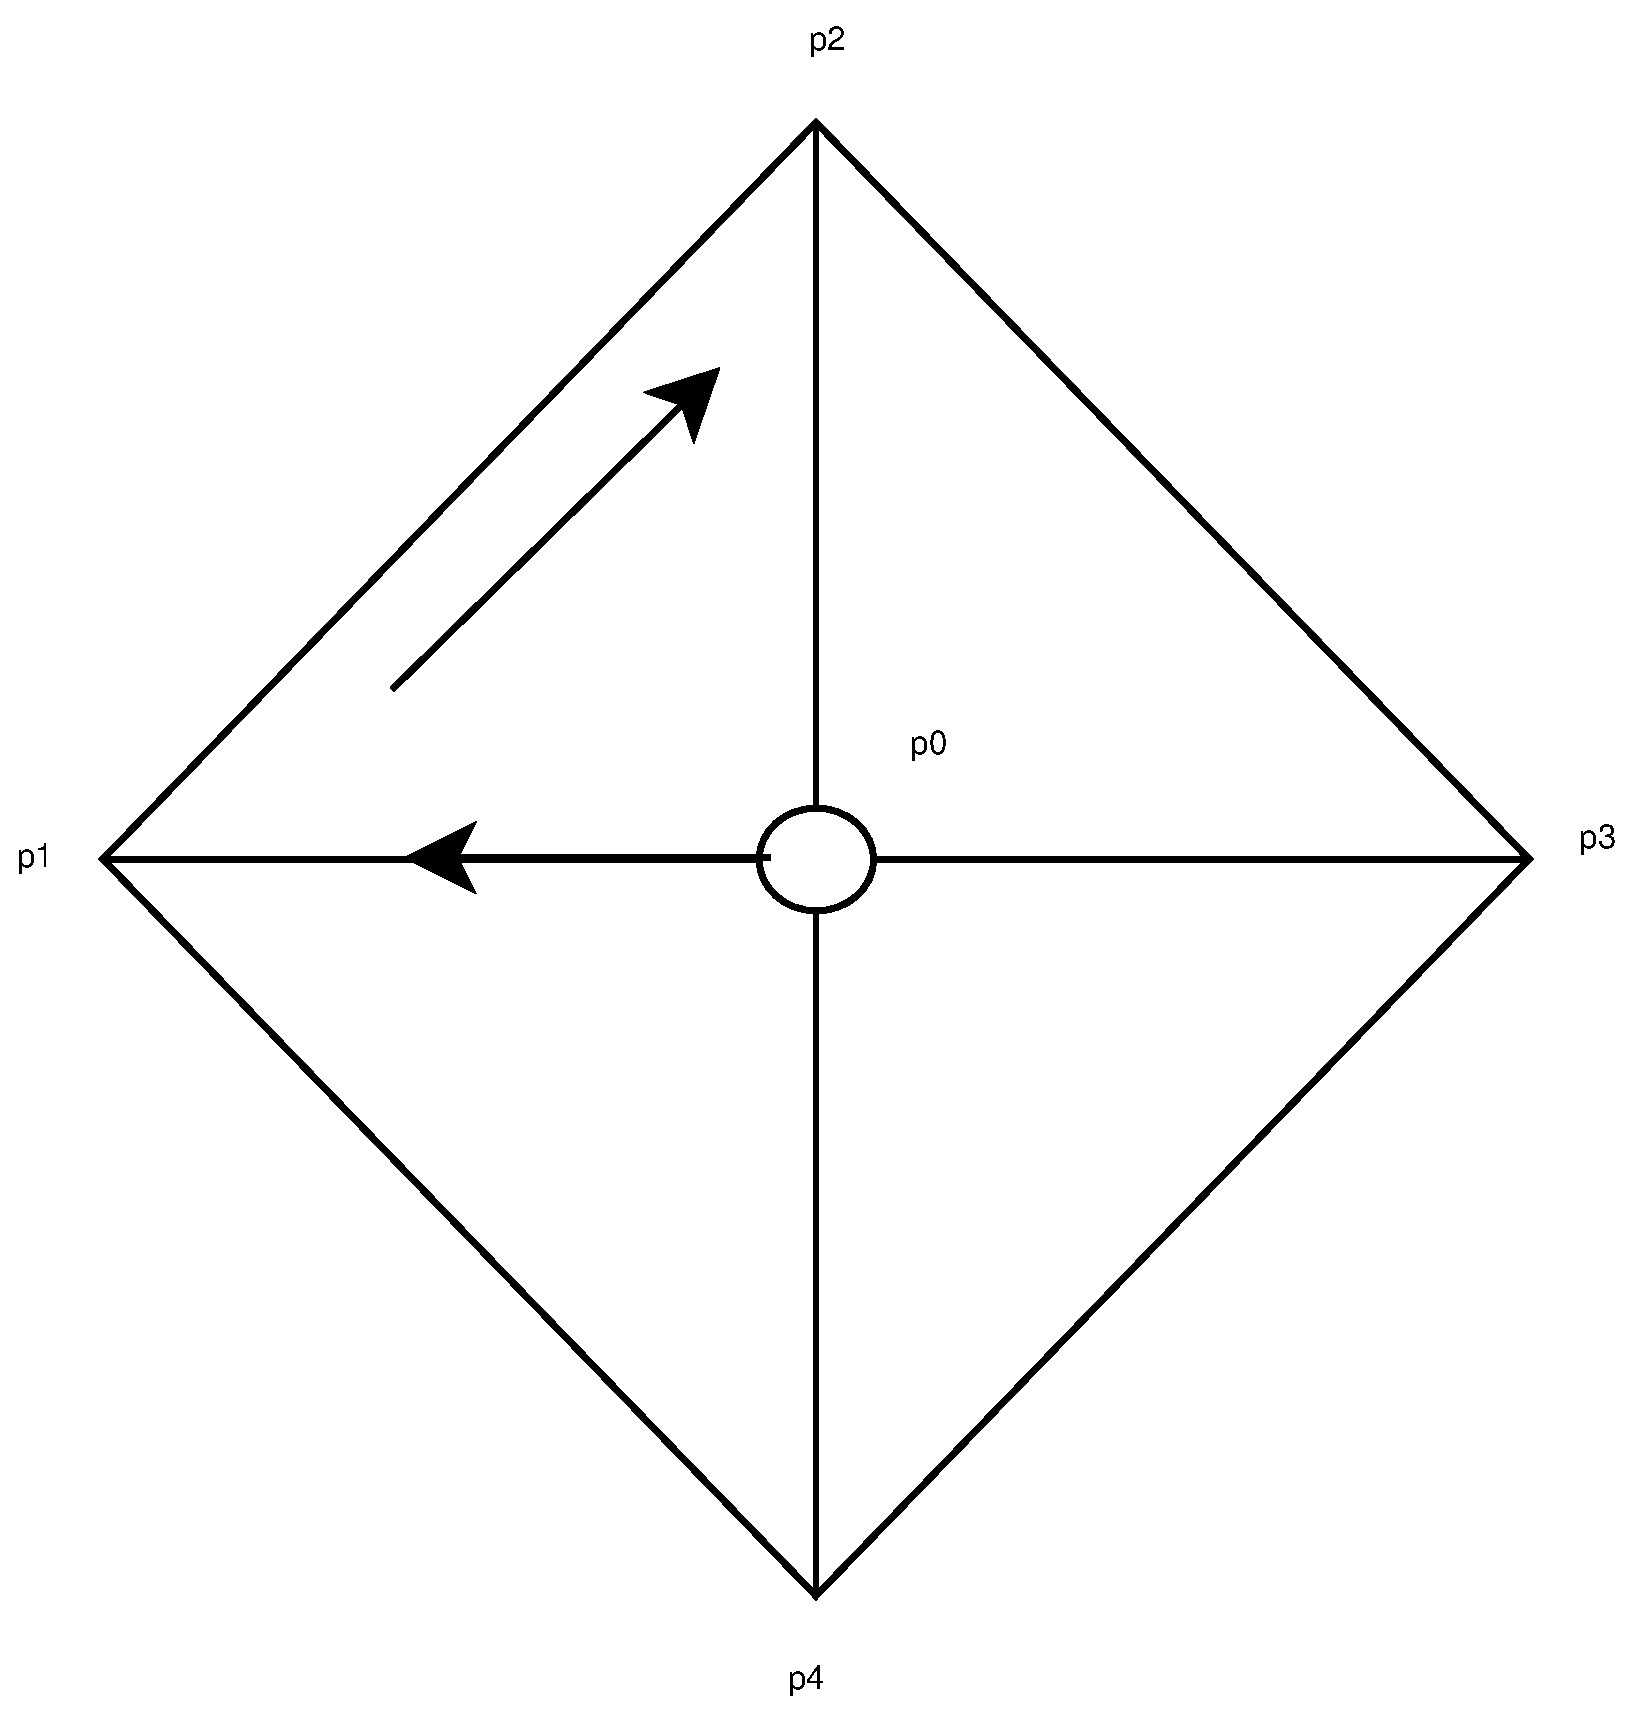
\includegraphics[width= 0.5\textwidth]{Figures/fp.eps}
\caption{Strategy for the fixed flight plan}
\label{f:fp}
\end{figure}

The basic logic of how it works is explained as follows:
Suppose the \ac{UAV} always starts from waypoint $p_0$. If it does not start from $p_0$, set $p_0$ as the stand by waypoint. Design four blocks which are denoted as ``go $p_1$'', ``go $p_2$'', ``go $p_3$'' and ``go $p_4$'' respectively. 

While executing the four blocks, it also executes an exception condition. Suppose the \ac{UAV} starts from $p_0$, now it goes to $p_1$. During this process, it will also run 
the following exception conditions:
\begin{enumerate}
\item if $\psi_v<0$, execute ``go $p_4$''.
\item if $\psi_v>0$, execute ``go $p_2$''.
\end{enumerate}
%
where $\psi_v$ is the heading angle generated by the vision algorithm.
If the \ac{UAV} is going from $p_1$ to $p_2$, then it also executes the following exception conditions:
\begin{enumerate}
\item if $\psi_v<0$, execute ``go $p_1$''.
\item if $\psi_v>0$, execute ``go $p_0$''.
\end{enumerate}



